% !TeX root = ../main.tex
% Add the above to each chapter to make compiling the PDF easier in some editors.

\chapter{Approach}\label{chapter:approach}
This chapter provides insight into the approach taken to run the schedule experiments. First, the framework used for the experiments is introduced, giving an overview of its functionality and of the required modifications performed on the framework itself and on the platforms upon which it was employed. Then, a preliminary examination of the two platforms is performed, including a study and analysis of their thermal behavior. This serves as a basis for the upcoming schedule experiments.
\section{Framework}
The evaluation of the various schedules generated by the GMPT algorithm requires a highly controlled environment. Since the temperature measurements of the processor are of paramount importance when comparing the results of the different algorithms, it needs to be ensured that, while the schedules are running, interference by other unrelated processes is minimal. Therefore, a special software setup is required. While open-source frameworks which were specifically designed to prototype real-time scheduling algorithms are available, they do not fully support the required functionality (such as custom frequency scaling). This has led to the implementation of a new framework by L. Bersentes \cite{Bersentes2017} which provides the required features and will be used within the scope of this thesis.
\subsection{Architecture}
The framework is implemented as a series of threads each of which represent one component within the process management system and functions as a full-scale simulation of it. \autoref{fig:i_arch} illustrates the Architecture of the framework.\\
The main building blocks, each of which run in their own thread, are: 
\begin{itemize}
\item \textbf{Main:} This component offers all the basic functionality such as initialization, reading input parameters as well as the creation of all other threads. Once all threads have started the simulation of the given schedule begins and this component sleeps throughout the entire experiment to minimize its performance impact. It is therefore completely inactive for the duration of the simulation.\\
\begin{figure}[H]
  \centering
  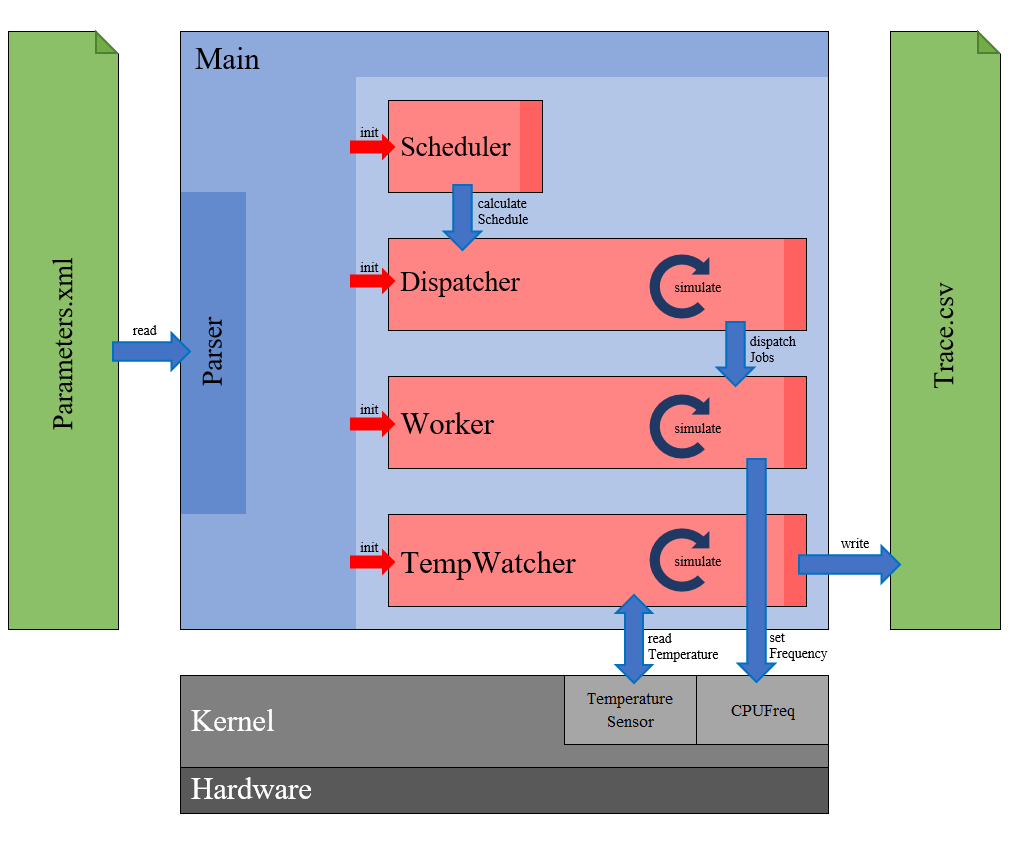
\includegraphics[height=12cm]{figures/arch}
  \caption[Architecture]{Framework Architecture}\label{fig:i_arch}
\end{figure}
\item \textbf{Scheduler:} This component is responsible for scheduling decisions. As it currently only supports static scheduling approaches, all scheduling decisions can be determined beforehand. This results in a minimal overhead as the thread is able to exit almost instantly, finishing much earlier than the actual simulation.
\item \textbf{Dispatcher:} This component is in charge of triggering all the jobs at the appropriate moment in time. Unlike in the case of the scheduler, the dispatcher needs to be active throughout the simulation as it needs to release the jobs by communicating with the worker. Even though all job parameters are known prior to execution it needs to be ensured that these parameters are actually enforced, otherwise there would be no guarantee that constraints such as period length apply. 
\item \textbf{Worker:} This component is used to manage all job related functions and represents one CPU core. It’s primary purpose is to execute the jobs released by the dispatcher and to do so by forcing the highest possible workload on a CPU core. It is furthermore responsible for switching between idle and active states (when idle states are part of the schedule) and for changing to the different CPU frequencies within one period.
\item \textbf{TempWatcher:} This component is used to monitor the CPU temperature throughout the entire simulation. The functionality has its own thread assigned to it to ensure that these measurements can be performed regularly and independently of the current state of the other components.
\end{itemize}
\begin{figure}[htpb]
  \centering
  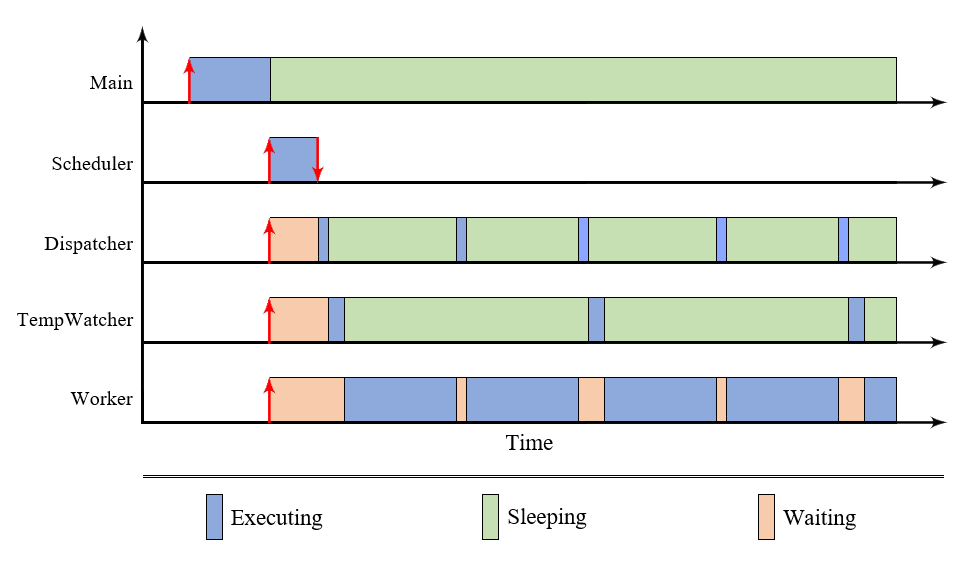
\includegraphics[height=8cm]{figures/frmw_sched}
  \caption[Framework Schedule]{Framework Thread Schedule}\label{fig:i_frmw_schd}
\end{figure}
An exemplary execution of these main components on a single core can be seen in \autoref{fig:i_frmw_schd} (the threads are sorted by their priority, Main having the highest priority).
\subsection{Platform Adjustments}\label{chap:plat_adj}
The GMPT algorithm will be evaluated on two different hardware platforms to analyze its feasibility. While the framework can run entirely inside the userspace, which implies high portability, it still relies on certain functionality provided by the kernel. Consequently some changes to the framework still have to be made when employing this framework in heterogenous environments.
\subsubsection{Platform: Notebook}
The first hardware platform upon which the GMPT algorithm will be tested is the LENOVO IdeaPad U330p operating an Intel Core i5-4210U and running Ubuntu 14.04 LTS.\\
\hspace*{0.5ex}\hspace{0.5ex} The very first step is to disable the integrated Intel P-State driver which does not provide control over the userspace governor and therefore would not allow to implement the custom frequency scaling that is required. Additionally the location of the kernel interfaces needs to be adapted and the available settable frequencies need to be added to the framework.\\
\hspace*{0.5ex}\hspace{0.5ex} A common way to set the CPU frequencies is via shell commands and this is also approach that has been implemented in the framework. While this approach may be simple and easy to implement, measurements (\autoref{fig:i_cmd_tim}) have shown that the execution of this command take a considerable amount of time (at times more than 1 ms) which may stall the execution of the job themselves therefore affecting the temperature development. This is especially problematic since the schedule provided by GMPT may only require the CPU to run at a certain frequency for 1 ms. The time it takes for the CPU to physically switch between frequencies is reported to be within the tens of microseconds \cite{intel_formula,Skadron,Semeraro}, arguably negligible compared to the time spent executing the command. The outlined problem has called for an improvement of this approach.\\
\begin{figure}[H]
  \centering
  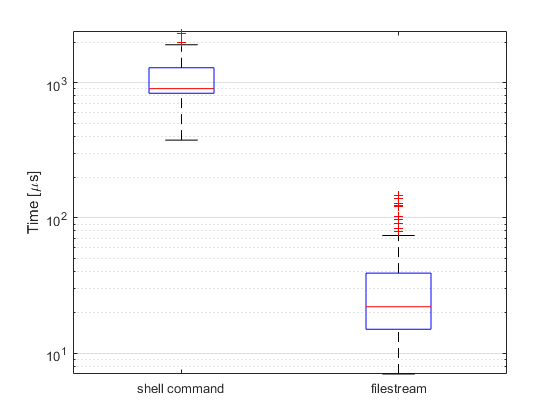
\includegraphics[height=7cm]{figures/cmd_time}
  \caption[Command Time]{Execution time of the two frequency switch implementations}\label{fig:i_cmd_tim}
\end{figure}
Still using the same kernel interface, instead of resorting to shell commands, I chose to communicate with it directly by the filestreams available in C++. As \autoref{fig:i_cmd_tim} illustrates, the performance was  increased by more than an entire order of magnitude, which should result in better confidence in the results.
\subsubsection{Platform: Raspberry Pi 3B}
To further improve the trust in the experimental results, the GMPT algorithm should also calculate a schedule for the Raspberry Pi 3B. This platform employs a 1.2 GHz 64-bit quad-core ARMv8 CPU integrated within its BCM2837 SoC. Raspbian Jessie Lite was chosen as the OS as it is expected to have the least impact on the generated results and overall performance due to its minimal image.\\
 \hspace*{0.5ex}\hspace{0.5ex} The Raspberry Pi only supports one CPUFreq driver and while it does support the userspace governor, the only two frequency levels that can be set are the minimum (600MHz) and maximum (1.2GHz) frequency. This is not sufficient for our use-case because at least four equidistant levels are needed. The first possibility to be investigated was expanding the userspace governor to support more frequency levels by adding the functionality in the kernel. Once this new customized kernel was tested, it turned out that the functionality could not be added to it due to missing firmware support \cite{Robingroppe2016}. As an alternative it was discovered that the CPU frequency could be set by the vcmailbox driver. This driver is responsible for the communication between the processor and the VideoCore and provides an interface which can be used for the purpose of this thesis \cite{vcmailbox}. In light of the attempted kernel customization it was noticed that the frequency reported by the kernel was merely based on the governor settings and hence not measured. Due to this implementation incorrect frequencies were reported by the kernel when set using the vcmailbox driver. This led to the employment of vcgencmd (a function provided by the VideoCore firmware \cite{vcgencmd}) which determines the true CPU frequency via clock measurements. The tool further led to the verification that vcmailbox can set permanent frequency levels regardless of current CPU workload or active governor, overriding any influence it may have.
\subsection{Overhead Analysis}\label{chap:ohd_a}
To be able to accurately interpret the experimental results, the overhead introduced by the framework itself needs to be considered. Due to disruptions by other threads and by certain instructions like the frequency change, the Worker won't be able to be active for the entire experiment. This overhead can be attributed to three main factors:
\begin{itemize}
\item \textbf{Job Dispatching:} This is expected to have the least overall impact since it simply manages a list of jobs. The Dispatcher runs in its own thread and therefore is still considered in this analysis.
\item \textbf{Temperature Measurements:} These are heavily platform dependent since the speed at which the measurements can be performed mostly depends on the built-in sensor.
\item \textbf{Frequency Changes:} As outlined in \autoref{chap:plat_adj}, the performance impact of the frequency switches is mostly implementation dependent. The adjustments made to the framework regarding this procedure are taken into account in this analysis.
\end{itemize}
Based on a 60 second experiment, the overhead introduced by these influences has been recorded. The average time consumed by single instances of such interruptions can be seen in \autoref{tab:t_ohd}.\\
\begin{table}[H]
 \centering
 \caption[Overhead]{Average overhead introduced by the framework}\label{tab:t_ohd}
 \begin{tabular}{||l | c | c||} 
 \hline
  & Notebook & Raspberry Pi 3B \\ [0.5ex] 
 \hline\hline
 Avg. Job Dispatch [$\mu s$] & 1.38 & 16.37 \\
 \hline
 Avg. Temp. Check [$\mu s$] & 7221.45 & 587.02 \\
 \hline
 Avg. Freq. Change [$\mu s$] & 27.64 & 6308.34 \\
 \hline
\end{tabular}
\end{table}
With the default settings of the framework (under which all experiments were run), the Dispatcher runs ten times per second. Considering the measured times, in a one minute experiment this amounts to approximately 830 $\mu s$ (~0.001\% of 60s) on the Notebook and 9820 $\mu s$ (~0.01\% of 60s) on the Raspberry Pi. This is not expected to have a major impact on the validity of the results.\\
\hspace*{0.5ex}\hspace{0.5ex} The temperature is measured five times per second (with default framework settings). In a 60 second experiment this results in overall 2.2 s (~3.6\% of 60s) on the Notebook and 176 ms (~0.3\% of 60s) on the Raspberry Pi. On both platforms this has a considerably bigger impact than the Dispatcher. However, this task has been assigned to a different core and should therefore not interrupt the Worker thread, minimizing its impact.\\
\hspace*{0.5ex}\hspace{0.5ex} The frequency switches show the biggest discrepancy between the two platforms. The actual impact this has on the overall execution heavily depends on the schedule used. If a schedule performs many frequency switches, the effect will be much more pronounced. On the Notebook this is expected to be less of an issue since the switch itself is performed fairly quickly, on the Raspberry Pi, however, this can severely impact the results due to the large amount of time dedicated to switching frequencies. The current implementation on the Raspberry Pi relies heavily on the driver provided by the OS (see \autoref{chap:plat_adj}) and steps taken to alleviate this problem have been mostly unsuccessful. This may be especially problematic if the timeslots within a schedule are very short and it needs to be taken into account when evaluating the results of future experiments on the Raspberry Pi (this does not affect the thermal profiles, as no frequency changes are performed there).
\section{Experiments}\label{t_prof}
The goal of the experiments is to provide thermal measurements for various schedules. This data is subsequently used to analyze different algorithms and compare them side-by-side.\\
\hspace*{0.5ex}\hspace{0.5ex} The framework that would ultimately be used to run the schedules was chosen on the basis of its high portability and due to the required functionality that was already implemented in it. For a first platform to test the framework and simulate the schedules, a notebook was chosen as it was readily available, was running a Linux distribution and did not have much additional software installed on it which could disrupt a smooth schedule simulation.  As a second platform to run and verify the schedules, the Raspberry Pi 3B was chosen. Here the framework could easily be run without any interference potentially caused by fans or heat sinks while still providing the commodity of an ordinary operating system. This lightweight OS also promised to generate easily reproducible and reliable temperature measurements due to its lack of a graphical user interface and consequently the lack of background calculations needed to support it.\\
\begin{figure}[H]
  \centering
  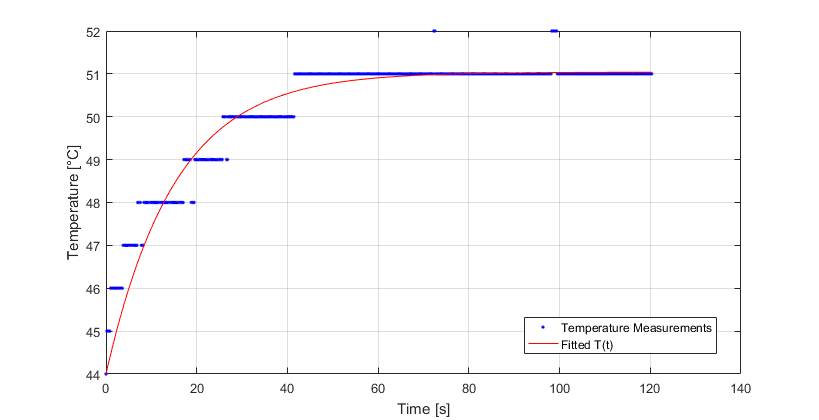
\includegraphics[height=7cm]{figures/temp_fit}
  \caption[Function Fit]{T(t) fitted to temperature measurements}\label{fig:i_fit}
\end{figure}
The goal of all evaluated algorithms is the peak temperature minimization within hard real-time constraints. The highest measured temperature may not be an accurate representation of the peak temperature as it may be too low due to unexpected interference or it simply has not yet been reached by the end of the experiment. Preliminary test runs have shown that for both platforms and most schedules $T^\infty_m$ is reached after about 60 seconds, hence all experiments ran for this duration, however, a better estimate of the peak temperature would still be desirable. Consequently the model presented in \ref{gmpt} is employed by fitting the function \eqref{eq:model} to the temperature measurements (\autoref{fig:i_fit}), this should return a more precise value for $T^\infty_m$. To further improve confidence in the results and detect possible outliers which may sabotage the data integrity, every experiment was run 10 times. In addition to these precautionary measures all of the experiments were performed in the same controlled environment under a constant ambient temperature. During the simulations, the platforms were dedicated entirely to the framework and no other work was performed on them.
\subsection{Platform Frequency Ranges}
The two platforms used for the experiments do not provide the same flexibility in their frequency settings. This and the need to limit the possible options available to the GMPT algorithm (to avoid overwhelming complexity) has led to the decision of constraining the settable frequencies to 4 equidistant levels denoted as 0.4, 0.6, 0.8, 1 and a 5th operating mode 0 which represents the idle state.\\
\begin{figure}[H]
  \centering
  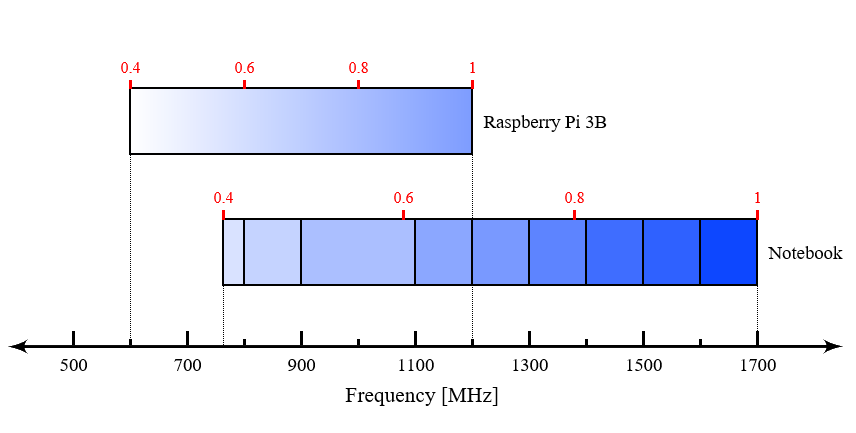
\includegraphics[height=7cm]{figures/freq_ranges}
  \caption[Frequency Ranges]{Frequency Ranges of the two hardware platforms}\label{fig:i_frq}
\end{figure}
\autoref{fig:i_frq} provides a comparison of the two frequency ranges available for the employed platforms. The first observation that can be made is that the notebook has a wider frequency range available. Even though the smallest possible frequency does not reach as low as the Raspberry Pi's range, this allows for more overall flexibility. Consequently the notebook has the ability to react more aggressively in certain situations. This possibility for drastic changes in the current frequency can be a great tool to influence the temperature development more swiftly and responsively, however, it also results in an increased performance variance which may be challenging to handle in time constrained systems. It should further be noted that only a very specific set of discrete frequency steps are available as settings. This leads to the problem that the frequency steps denoted as 0.6 and 0.8 may not be available as actual settings (as it is the case for the notebook platform). In such a case the frequency closest to the desired setting is chosen by the framework. In contrast to this, the mailbox driver employed on the Raspberry Pi allows to set a very large amount of frequency levels. Here the frequency can be specified down to the kHz level. This allows for very accurate frequency adjustments within this overall smaller range. In this current use-case such accuracy is not really required and would actually be highly problematic if used to its full extend. Apart from rendering the schedule optimization very costly, the large amount of available frequency options could also entail a high number of frequency switches resulting in a very large overhead used entirely for the switching process. Therefore the schedules for this platform have also been restricted to use four frequency levels. On the Raspberry Pi these frequency settings are precisely available due to the given step granularity and don't need to be approximated like on the notebook.
\subsection{Thermal Profiles}
Before the GMPT algorithm is able to calculate any schedules for a given platform, thermal profiles of that platform have to be provided. These profiles give an insight on how temperature development is affected by a specific frequency setting. This information is crucial to understanding how the processor will behave for a certain schedule and is therefore important when making according predictions to optimize it.\\
\hspace*{0.5ex}\hspace{0.5ex} These thermal profiles were determined by running schedules inside the framework at constant frequency settings. The first schedule (0) consisted of idle times only, here the frequency was set to the minimum and no calculation were performed during any period (i.e. the CPU was completely idle for the entire simulation). For the following simulations the four equidistant frequency settings 0.4, 0.6, 0.8 and 1 were used.\\
\subsubsection{Thermal Profile: Notebook}
Additionally to the adjustments detailed in \ref{chap:plat_adj} the built-in fan was disabled to get more accurate and reliable readings regarding the temperature dissipation. Other hardware cooling devices (such as the heat sink) were not removed in order not to corrupt the platform integrity. Since the focus lied on the performance of different scheduling algorithms on a single core, all unused cores were constantly set to their lowest possible frequency and kept at idle.\\
\begin{table}[H]
 \centering
 \caption[Thermal Profile Notebook]{Average results for notebook platform}\label{tab:t_tp_n}
 \begin{tabular}{||c | c | c||} 
 \hline
 Frequency Setting & Average $T^\infty_m$ [$^{\circ}$C] & Average $R^2$ \\ [0.5ex] 
 \hline\hline
 0 & 43.933 & - \\
 \hline
 0.4 & 47.183 & 0.721 \\
 \hline
 0.6 & 48.895 & 0.812 \\
 \hline
 0.8 & 51.322 & 0.900 \\
 \hline
 1 & 65.680 & 0.860 \\
 \hline
\end{tabular}
\end{table}
The average results for $T^\infty_m$ can be seen in \autoref{tab:t_tp_n} together with their average coefficient of determination $R^2$ which serves as an indicator of how closely the data matches our given model. $R^2$ is not reported for the idle measurements since it does not apply here (the idle temperature is constant).\\
\hspace*{0.5ex}\hspace{0.5ex} \autoref{fig:i_tp_n} displays the thermal profile for the notebook platform including the results for idle and the four frequency settings with maximum workload. This analysis shows a considerable jump in temperature for the highest frequency level. This can be explained by the relation \cite{intel_formula} $$P = C V^2 F,$$ where \(P\) is the power dissipation, \(C\) is the capacitance, \(V\) is the voltage and \(F\) is the frequency at which the integrated circuit is operating. While the frequency on its own affects the power dissipation linearly, the CPU implicitly adapts the voltage accordingly (higher frequency also means higher voltage). Therefore, for each experiment, voltage and frequency were increased, which, when combined, result in a cubic influence on power dissipation, ultimately leading to the cubic behavior of the temperature development. The data provided for the idle run should not be considered as a part of this function since it differs in CPU utilization from the other four settings.
\begin{figure}[H]
  \centering
  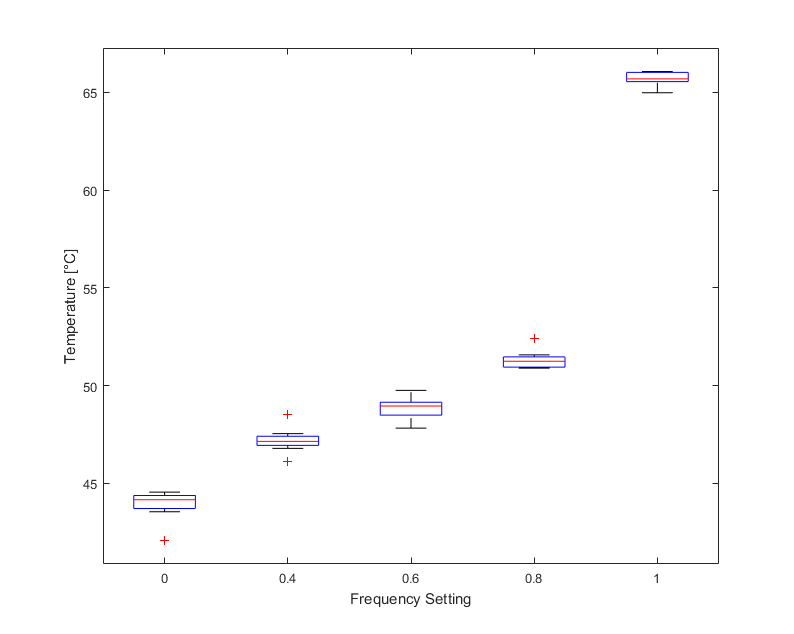
\includegraphics[height=7cm]{figures/profile_notebook}
  \caption[Thermal Profile Notebook]{Thermal profile of the notebook platform}\label{fig:i_tp_n}
\end{figure}
\subsubsection{Thermal Profile: Raspberry Pi 3B}
Unlike in the case of the first platform, hardware cooling devices like fans and heatsinks are not preinstalled on the Raspberry Pi 3B. The measurable results were therefore expected to be a better representation of the actual processor's thermal performance. The CPU on this platform includes four cores but the mailbox driver used to set the frequencies can only set the frequencies of all cores at once. The frequency scaling therefore also affected the other three cores but since they were idle only a small impact on the overall thermal behavior was expected.\\ \hspace*{0.5ex}\hspace{0.5ex} The average results for the Raspberry Pi platform and the associated $R^2$ values are reported in \autoref{tab:t_tp_pi}.\\
\begin{table}[H]
 \centering
 \caption[Thermal Profile Raspberry Pi]{Average results for Raspberry Pi 3B}\label{tab:t_tp_pi}
 \begin{tabular}{||c | c | c||} 
 \hline
 Frequency Setting & Average $T^\infty_m$ [$^{\circ}$C] & Average $R^2$ \\ [0.5ex] 
 \hline\hline
 0 & 45.087 & - \\
 \hline
 0.4 & 49.198 & 0.811 \\
 \hline
 0.6 & 50.255 & 0.797 \\
 \hline
 0.8 & 51.965 & 0.914 \\
 \hline
 1 & 52.792 & 0.933 \\
 \hline
\end{tabular}
\end{table}
The profile for the Raspberry Pi depicted in \autoref{fig:i_tp_pi} shows a clear difference from the notebook profile. The maximum frequency does not cause the big temperature increase observed on our first platform. In order to exclude possible interference caused by other cores the experiments were run a second time with three of the four cores completely turned off, however this resulted in a temperature increase of approximately 6$^{\circ}$C for every frequency setting (keeping the relative temperature changes constant). An evaluation of the CPU utilization returned a workload of >97\% throughout the simulation, which is identical to the notebook data. Extending the simulation time also yielded no significant changes in the thermal profile. Since the temperature changes for similar frequencies were also small on the first platform it was ultimately concluded that the lack of major temperature changes is the result of a smaller frequency range and a lower available maximum frequency. This can not be fully verified due to the lack of data such as the thermal design power specification of the ARM Cortex-A53 (datasheet not publicly available). While this smaller temperature range may render the comparison of different approaches more challenging, a smaller spread of the experimental results within every frequency setting can be observed. This implies a more accurate temperature control via the frequency setting and is expected to improve overall data quality for the upcoming algorithm tests.\\
\begin{figure}[htpb]
  \centering
  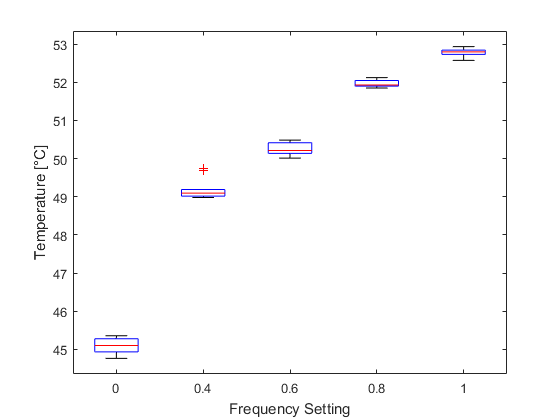
\includegraphics[height=7cm]{figures/profile_pi}
  \caption[Thermal Profile Raspberry Pi 3B]{Thermal profile of the Raspberry Pi 3B}\label{fig:i_tp_pi}
\end{figure}